\documentclass[font=default]{mpltx}
\usepackage{bm, ctex}
\usepackage{subfigure}
\usepackage{multirow}
% 以下至 \begin{document} 都仅是本文件为了方便额外定义的命令, 写报告时不需要.
\hypersetup{colorlinks=false}% 超链接带颜色
\usepackage{xcolor}
% 以上是本文件为了方便额外定义的命令, 写报告时不需要.
\linespread{1.5}
\begin{document}

\title{脉冲核磁共振与成像} % 切合报告内容, 简短明确, 可以不同于讲义
\author{MaskedName} % 这里 \emailphone 一定要紧跟在 \author 后方
\emailphone{MyMail@stu.pku.edu.cn}{Tel}
% 如果改用 \email 则仅需要邮箱参数
\affiliation{北京大学物理学院\quad 学号: StudentID}
\date{\zhdate{2023/11/29}}
\begin{abstract}
  核磁共振成像是通过核磁共振进行成像的一种技术,因具有非侵入性,被广泛运用于医学监测领域,具有无辐射、高分辨率和能够提供分子内部结构信息的优点。本实验旨在探究不同浓度的CuSO$_4$溶液对弛豫时间的影响,并通过成像实验探究$T_2$加权的原理。实验结果显示,随着溶液浓度的增加,图像的亮度逐渐降低,这表明高浓度溶液中的弛豫时间较短,导致信号衰减较快。通过本次实验能对脉冲核磁共振成像有一个更加直观的了解,并且明白影响成像结果的各种因素。
\end{abstract}
\keywords{脉冲核磁共振,自旋回波,核磁共振成像,弛豫时间,CuSO$_4$溶液}

\maketitle

\section{引言}
核磁共振(NMR,Nuclear Magnetic Resonance)是一种通过观察原子核在特定频率的射频场中发生共振吸收的现象的技术。在原子核激发和退激发过程中,其弛豫时间受到物质种类、环境等多种因素的影响。通过施加梯度磁场,可以检测到原子核发射的电磁波,进而通过空间编码获得物体内部的结构图像。

核磁共振技术最初由Isidor Rabi于上世纪30年代发现。他观察到在磁场中的原子核会沿磁场方向有序平行排列,而在施加无线电波后,原子核的自旋方向会发生翻转\cite{rabi1938new}。随后,人们发现水分子中的氢原子可以发生核磁共振,并利用这一现象获取生物体内的水分子分布信息,从而了解内部结构。在1966年,Raymond Damadian通过测量核磁共振的弛豫时间首次将小鼠的正常细胞与癌细胞区分开来。随后,P.C. Lauterbur于1973年开发了核磁共振成像技术\cite{lauterbur1973image},并与Peter Mansfield共同荣获了2003年度诺贝尔生理学或医学奖。

目前使用的核磁共振仪器主要有连续波核磁共振波谱仪(CW-NMR)和脉冲傅里叶核磁共振仪(PFT-NMR)。前者操作简单,价格较低,但后者具有高灵敏度、短扫描时间以及可以测量弛豫时间的优点。因此,绝大部分核磁共振谱仪采用脉冲法,而核磁共振成像仪则普遍采用脉冲法\cite{book}。

本实验使用苏州纽迈分析仪器股份有限公司生产的EDUMR20-015V-I型核磁共振成像技术实验仪,测定三种浓度的CuSO$_4$溶液(0.5\%,1\%,2\%)的弛豫时间$T_1$和$T_2$。同时,通过浸泡在CuSO$_4$溶液中的不同形状的样品,获取核磁共振图像。最后,我们将0.5\%溶液试管放进1\%和2\%溶液试管,以探究$T_2$加权成像原理。通过这些实验,我们期望深入了解核磁共振技术在物质内部结构分析和成像方面的应用。
\section{理论\cite{book}}
\subsection{核磁共振基本原理}
  原子的的核磁矩在外磁场$\bm{B}_0$下产生分裂获得额外能量
	\begin{equation}
		\Delta E=\gamma \hbar mB_0,
	\end{equation}
	对于质子来说$m$的取值为$\pm1/2$,从而在外磁场下分裂成两个能级。
	从运动学的角度看,核磁矩的方向和外磁场并不保持一致,我们可以写出核磁矩的运动方程
	\begin{equation}
		\frac{{\rm d} \bm{\mu}}{{\rm d}t}=\gamma\left( \bm{\mu \times \bm{B}_0}\right) .
	\end{equation}
	
	角频率$\omega_0=\gamma B_0$称为拉莫尔(Larmor)频率,原子核以该频率绕磁场$\bm{B}_0$进动,核磁矩与$\bm{B}_0$的夹角$\theta$保持不变。若在垂直于$\bm{B}_0$的平面内加一以$\omega_0$旋转的磁场$\bm{B}_1$,则原子核会发生共振吸收,核磁矩与$\bm{B}_0$的夹角$\theta$会发生改变。
\subsection{宏观磁矩和弛豫过程}
  实验中观察到的是大量核磁矩的统计平均,在宏观的非磁性物体中,磁矩的取向是随机的,宏观上不表现出任何磁性。在磁场$\bm{B}_0$的作用下,每个小磁矩绕着$\bm{B_0}$的方向旋进,彼此之间的相位是随机的,于是宏观磁矩$\bm{M}=\bm{M}_0$沿磁场方向。而在射频场$\bm{B}_1$的作用下,$\bm{M}$将会偏离$z$轴,从而同时具有$\bm{M}_z$和$\bm{M}_{xy}$分量,这意味着各个磁矩的相位有了一定的一致性。撤去射频场后,由于自旋-晶格相互作用和自旋-自旋相互作用,核磁矩之间的相位会逐渐趋向无序,即$\bm{M}_{xy}\to 0$,宏观磁矩会趋向$\bm{M}_0$。宏观磁矩随时间的演化关系为
	\begin{equation}
    \begin{aligned}
      M_z&=M_0+\left( M_z^0-M_0\right) e^{-\frac{t}{T_1}},\\
		  M_{xy}&=M_{xy}^0e^{-\frac{t}{T_2}}.
    \end{aligned}
	\end{equation}
	
	其中$M_z^0,M_{xy}^0$是$t=0$时$M_z,M_{xy}$的值,$T_1,T_2$分别为纵向弛豫时间和横向弛豫时间,且一定有$T_1>T_2$。实际上,由于外加磁场的不均匀性(这等效于一个弛豫时间为$T_2'$的弛豫),只能测得等效的横向弛豫时间$T_2^*$,且有
	\begin{equation}
		\frac{1}{T_2^*}=\frac{1}{T_2}+\frac{1}{T_2'}.
	\end{equation}

  所以我们有
	\begin{equation}
		T_1>T_2>T_2^*.
	\end{equation}
\subsection{核磁共振成像}
核磁共振成像的关键在于对空间信息的编码与反演。在三维成像系统中,该过程可以分为三个关键步骤:

\subsubsection{$\hat{\bm{z}}$方向截面选取}

为了选择$\hat{\bm{z}}$方向上的横截面,我们通过在$\hat{\bm{z}}$方向加一线性梯度磁场$G_z\bm{z}$,并调节射频场的频率为

\begin{equation}
  \omega(z_1) = \gamma B(z_1) = \gamma(B_0 + G_z z_1),
\end{equation}

式中$G_z$为一常量。这样只有位于$z=z_1$附近的原子核会发生共振,其他位置的核处于非共振状态,因而对NMR信号无贡献(如\autoref{fig:z_dir} 所示),且$G_z$选取越大,射频脉冲圆频率的带宽就越窄,$z$方向的分辨率就越高。
\begin{figure}
  \centering
  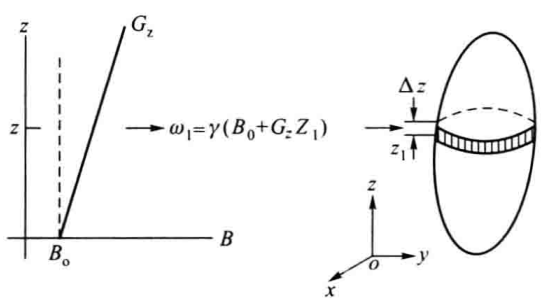
\includegraphics[width=0.4\linewidth]{fig/z_dir.png}
  \caption{z方向的梯度场和选层}
  \label{fig:z_dir}
\end{figure}

\subsubsection{$\hat{\bm{y}}$方向相位编码}

去除射频场和梯度场后,通过加与原磁场$B_0$方向相同,而强度大小沿$y$方向不相同的磁场$B_z =B(z_1)+ G_y y$,使得不同$y$处的核磁矩以不同的角频率进动
\begin{equation}
  \omega(y,z_1)=\gamma(B(z_1)+G_y y)=\omega(z_1)+\omega(y).
\end{equation}
经过作用时间$t_y$后,不同$y$处的核具有不同的相位
\begin{equation}
  \Phi_y = \Phi_0 + \omega(y)t_y ,
\end{equation}
从而实现了$y$方向的相位编码。

\subsubsection{$\hat{\bm{x}}$方向频率编码}

撤去梯度场$B_z = G_y y$后,再加$B_z = B(z_1)+G_x x$使得不同$x$处的核磁矩以不同的角频率进动
\begin{equation}
  \omega(x, z_1) = \gamma (B(z_1) + G_x x) = \omega(z_1) + \omega(x).
\end{equation}
这实现了$x$方向的频率编码。横断面上每一空间位置$(x,y)$都可以由其对应的$\Phi(y)$相位和频率$\omega(x)$来确定。

\subsubsection{反演原理}
在$xy$平面内的磁化强度矢量才可以转化为核磁共振信号,考虑到$\bm{M}_{xy}$围绕着$\bm{B}$进动,可以将$xy$平面内的磁化强度矢量随时间变化关系写为
\begin{equation}
  \bm{M}_{xy}(t)=(\bm{M}_{xy}^0e^{-\frac{t}{T_2}})e^{-i\omega t}.
\end{equation}
我们测量到的信号$S(t)$和$M_{xy}(t)$成正比,而磁化强度又和自旋原子核的数目成正比。令$\rho(x,y)$为自旋核的密度,则
\begin{equation}
  S(t) \propto \iint\rho(x, y)e^{-\frac{t}{T_2}} e^{i\omega t}{\rm d}x{\rm d}y
\end{equation}
对于一个确定的$t_y$,我们可以测得回波信号$S(t)$。通过改变$t_y$多次测量,我们得到一系列的回波信号$S(t_x, t_y)$。同时考虑到$x$方向频率编码和$y$方向相位编码的影响,我们有

\begin{equation}
S(t_x, t_y) =k \iint \rho(x, y) e^{i(\omega_x t_x + \omega_y t_y)}{\rm d}x {\rm d}y
\end{equation}

这里因为$e^{-t/T_2}$和$e^{i\omega(z_1)t}$对积分没有贡献,不影响我们的正比关系。$\omega_x$和$\omega_y$分别与$x$和$y$成正比。通过对$S(t_x, t_y)$进行傅里叶变换,我们可以得到核磁共振图像
\begin{equation}
  \rho(x,y)=h\iint S(t_x,t_y)e^{i(\omega_x t_x + \omega_y t_y)}\,{\rm d}t_x \,{\rm d}t_y
\end{equation}
实际不同位置处成像物质的$T_2$是不同的,上式可看作是$T_2$加权的核密度分布。增加$t$可使$T_2$的权重变大,从而使不同$T_2$的物质在核磁共振图像中的反差增强。这为我们提供了关于样品内部结构的空间信息。
\section{实验内容}
本实验采用苏州纽迈分析仪器股份有限公司生产的EDUMR20-015V-I型核磁共振成像技术实验仪,该仪器具有高度自动化的特点,只需简单地将样品放入设备中并操作相关软件即可进行实验。

实验开始时,按照以下步骤进行:

\begin{enumerate}
    \item 打开电脑电源、SPECTROMETER UNIT电源、RADIO FREQUENCY UNIT电源和GRADIENT UNIT电源。
    
    \item 等待设备温度达到预设温度(约等待90min),确保温度波动小于$0.01^\circ$C后,将标准样品放入样品台。
    
    \item 启动实验操作软件,准备进行实验。
\end{enumerate}

\subsection{采集FID信号}

根据仪器说明书的指引,调节各个增益参数和信息采集参数,校准共振频率,并扫描获得$\frac{\pi}{2}$和$\pi$脉冲宽度。使用SE序列观察回波信号。

\subsection{浓度为$2\%,1\%,0.5\%$的${\rm CuSO_4}$溶液测量弛豫时间}

随后,将浓度分别为$2\%,1\%,0.5\%$的${\rm CuSO_4}$溶液放入样品台。利用CPMG序列测量横向弛豫时间$T_2$,利用IR序列测量纵向弛豫时间$T_1$。

\subsection{核磁共振成像}

在完成弛豫时间测量后,打开成像软件。分别将不同形状的样品放入不同浓度的${\rm CuSO_4}$溶液中。根据软件的指导,利用核磁共振成像技术获取图像。

最后,将浓度为$0.5\%$的${\rm CuSO_4}$试管插入$1\%$和$2\%$溶液中,进行$T_2$加权成像。
\section{实验结果与分析}
\subsection{校准共振频率,扫描获得脉冲宽度}
调节各个参数后进行单次扫描,并使用软件自带的功能找到共振频率、扫描$90^\circ$和$180^\circ$脉冲宽度如\autoref{fig:reso_freq} 所示。得到共振频率
\begin{equation}
  f_0=21.977148\ {\rm Hz},
\end{equation}$90^\circ$和$180^\circ$脉冲宽度分别为
\begin{equation}
  \begin{aligned}
    \tau_{\pi/2}=18.0\ \mu {\rm s},\\
		\tau_{\pi}=38.0\ \mu {\rm s}.
  \end{aligned}
\end{equation}
\begin{figure}[htbp]
  \centering    %居中
  \subfigure[找到中心频率后的图像] %第一张子图
  {
    \begin{minipage}[b]{0.48\linewidth}
      \centering          %子图居中
      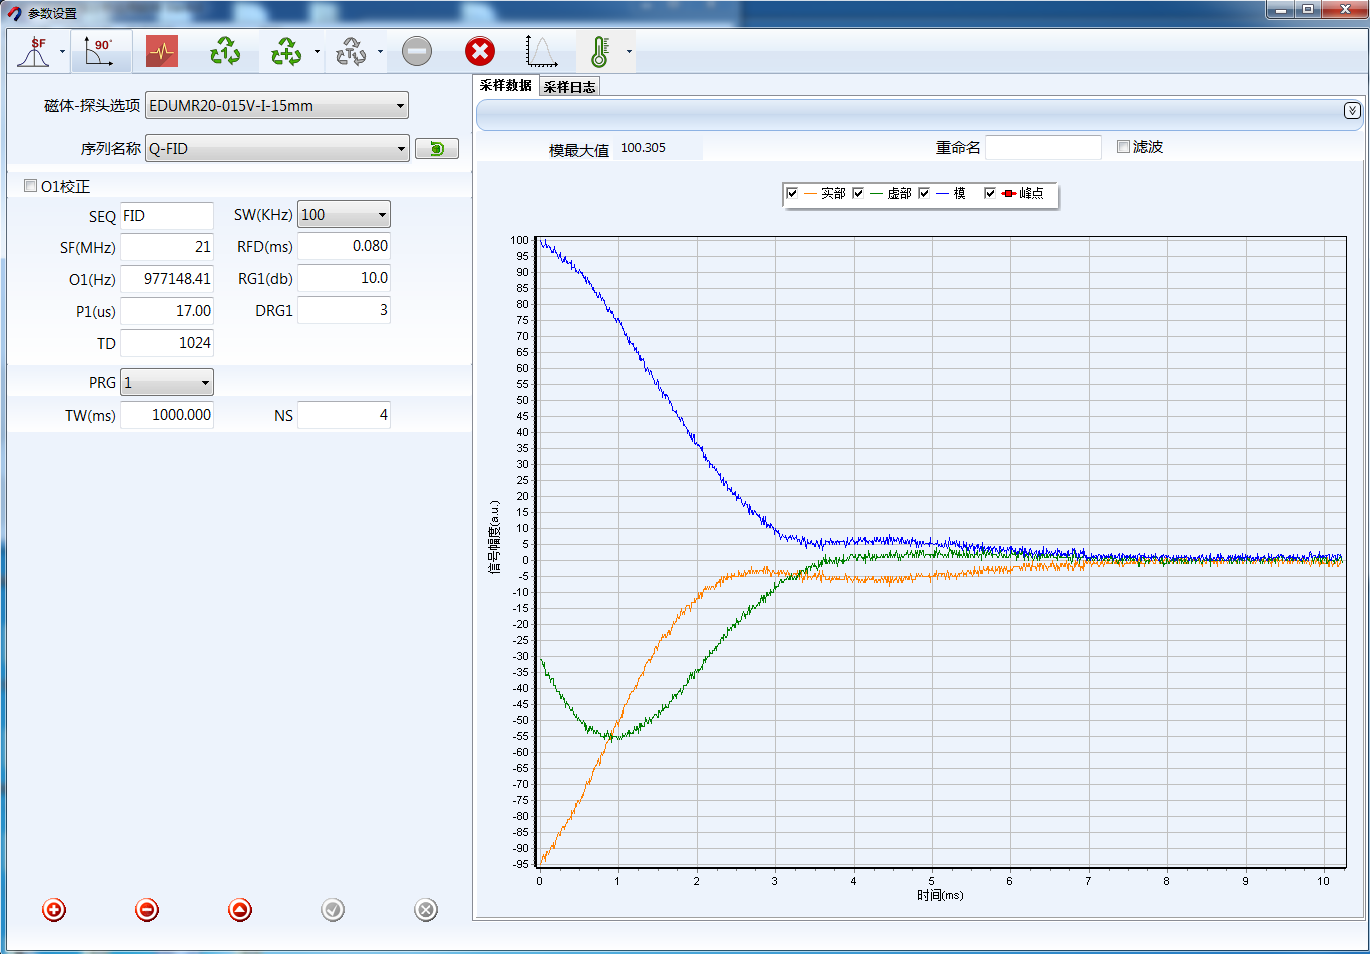
\includegraphics[width=\linewidth]{fig/central_freq.png}   %以pic.jpg的0.5倍大小输出
    \end{minipage}
  }
  \subfigure[确定硬脉冲脉宽] %第二张子图
  {
    \begin{minipage}[b]{0.48\linewidth}
      \centering      %子图居中
      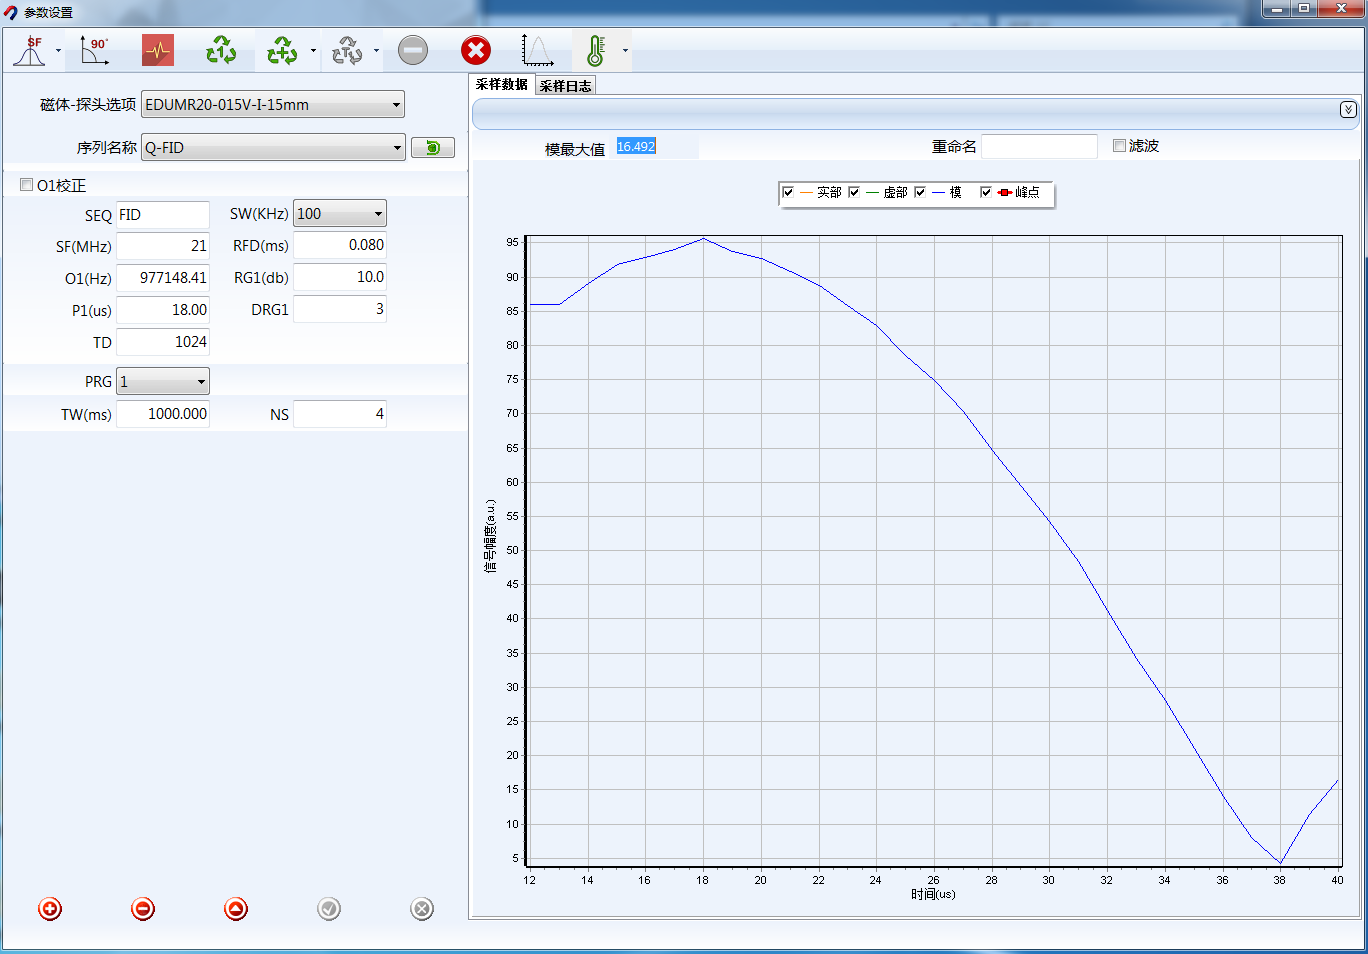
\includegraphics[width=\linewidth]{fig/freq_width.PNG}   %以pic.jpg的0.5倍大小输出
    \end{minipage}
  }
  \caption{校准共振频率,扫描获得脉冲宽度结果} %  %大图名称
  \label{fig:reso_freq}  %图片引用标记
\end{figure}
\subsection{测量不同浓度${\rm CuSO_4}$溶液的弛豫时间}
测量不同浓度的${\rm CuSO_4}$溶液的弛豫时间的结果如\autoref{fig:delaytime} 所示,程序已经将测量到的$T_2^*$转化为$T_2$,图上显示的就是最终测量结果。

可以观察到,在不论浓度的溶液下,均有$T_2 > T_1$。这与理论分析结果一致,符合核磁共振的基本性质。此外,若我们测量并比较$T_2^*$和$T_2$的结果(本报告中没有展示),我们发现二者之间存在较大的差异。这表明磁场的不均匀性对于横向弛豫时间的影响较大,因此在实际测量中必须考虑磁场不均匀性引起的影响。

\begin{figure}[]
  \centering    %居中
  \subfigure[浓度为$0.5\%$的${\rm CuSO_4}$溶液的弛豫时间] %第一张子图
  {
    \begin{minipage}[b]{0.48\linewidth}
      \centering          %子图居中
      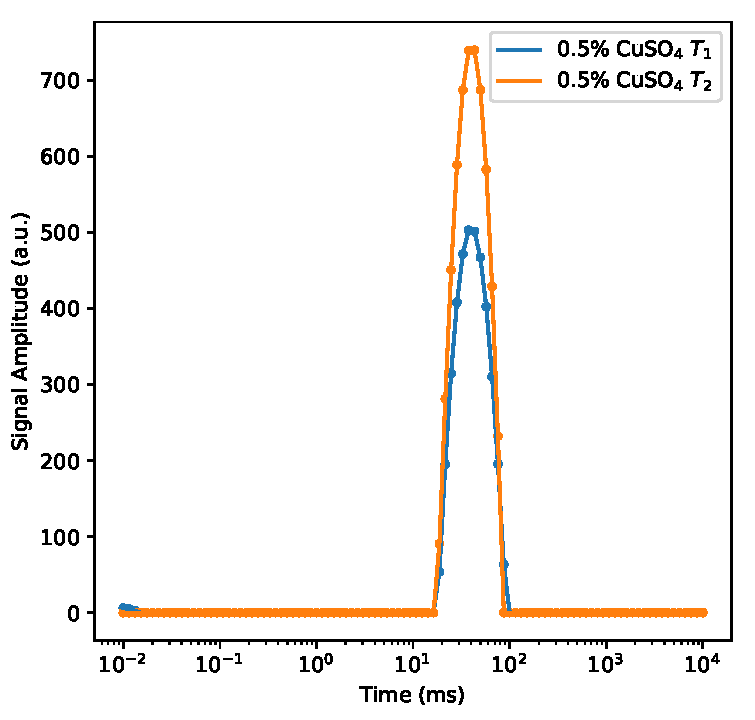
\includegraphics[width=\linewidth]{fig/0.5CuSO4.pdf}   %以pic.jpg的0.5倍大小输出
    \end{minipage}
  }
  \subfigure[浓度为$1\%$的${\rm CuSO_4}$溶液的弛豫时间] %第二张子图
  {
    \begin{minipage}[b]{0.48\linewidth}
      \centering      %子图居中
      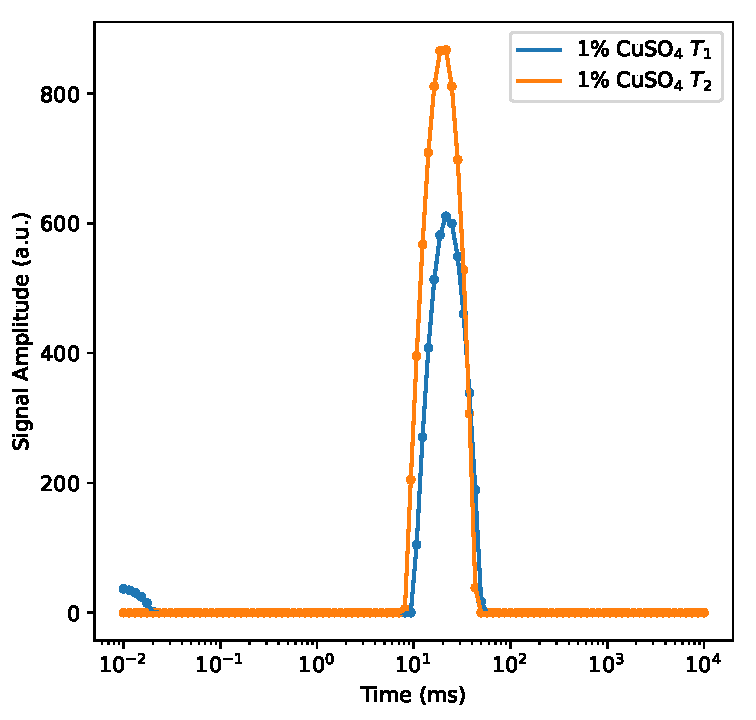
\includegraphics[width=\linewidth]{fig/1CuSO4.pdf}   %以pic.jpg的0.5倍大小输出
    \end{minipage}
  }
  \subfigure[浓度为$2\%$的${\rm CuSO_4}$溶液的弛豫时间] %第二张子图
  {
    \begin{minipage}[b]{0.48\linewidth}
      \centering      %子图居中
      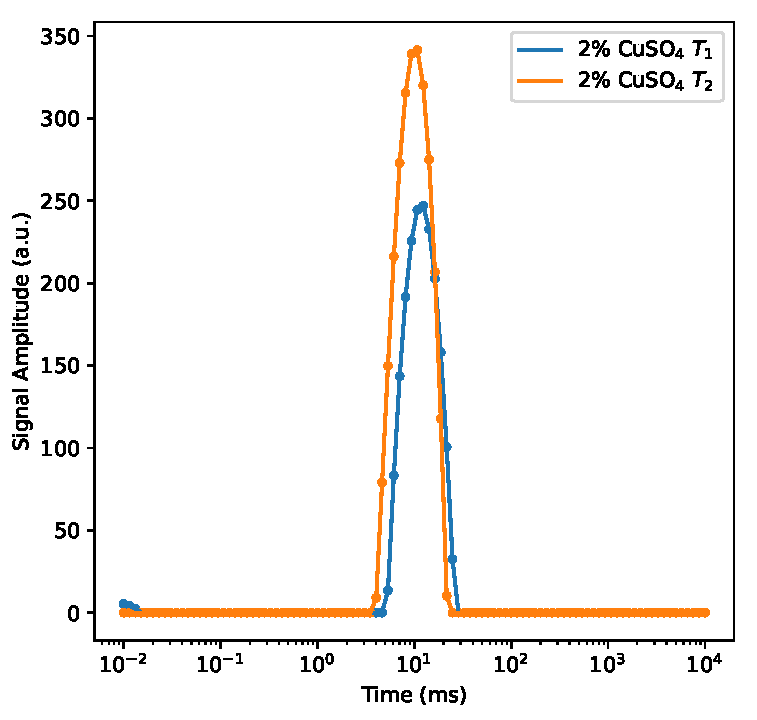
\includegraphics[width=\linewidth]{fig/2CuSO4.pdf}   %以pic.jpg的0.5倍大小输出
    \end{minipage}
  }
  \caption{不同浓度的${\rm CuSO_4}$溶液的弛豫时间} %  %大图名称
  \label{fig:delaytime}  %图片引用标记
\end{figure}

\autoref{tab:time} 列出了三种浓度的CuSO$_4$溶液的弛豫时间。
\begin{table}[]
    \centering
    \caption{不同浓度的${\rm CuSO_4}$溶液的弛豫时间。表中的“峰顶点时间”可以看作是$T_1$或者$T_2$的测量值。}
    \label{tab:time}
    \begin{tabular}{l|ccc|ccc}
      \hline\hline
      & \multicolumn{3}{c|}{$T_1$}&\multicolumn{3}{c}{$T_2$}\\\hline
      溶液浓度& 峰起始时间(ms)  & 峰顶点时间(ms)  & 峰结束时间(ms)   & 峰起始时间(ms)  & 峰顶点时间(ms)  & 峰结束时间(ms)  \\
    0.5\%  & 16.298 & 37.649 & 100.000 & 16.298 & 43.288 & 86.975 \\
    1\%    & 9.326  & 21.544 & 57.224  & 7.055  & 21.544 & 49.770  \\
    2\%    & 4.642  & 12.328 & 28.480  & 3.511  & 10.723 & 24.771 \\\hline\hline
    \end{tabular}
\end{table}
不同浓度的CuSO$_4$溶液提供了不同浓度的顺磁离子,这些离子将使得周围的局域磁场大大增强,从而减小弛豫时间。理论上来说,浓度越高的CuSO$_4$溶液,其提供的顺磁离子就越多,因此样品的弛豫时间就越短。\autoref{fig:diff_delaytime} 展示的结果就验证了这个理论。
\begin{figure}[]
  \centering    %居中
  \subfigure[纵向弛豫时间$T_1$] %第一张子图
  {
    \begin{minipage}[b]{0.48\linewidth}
      \centering          %子图居中
      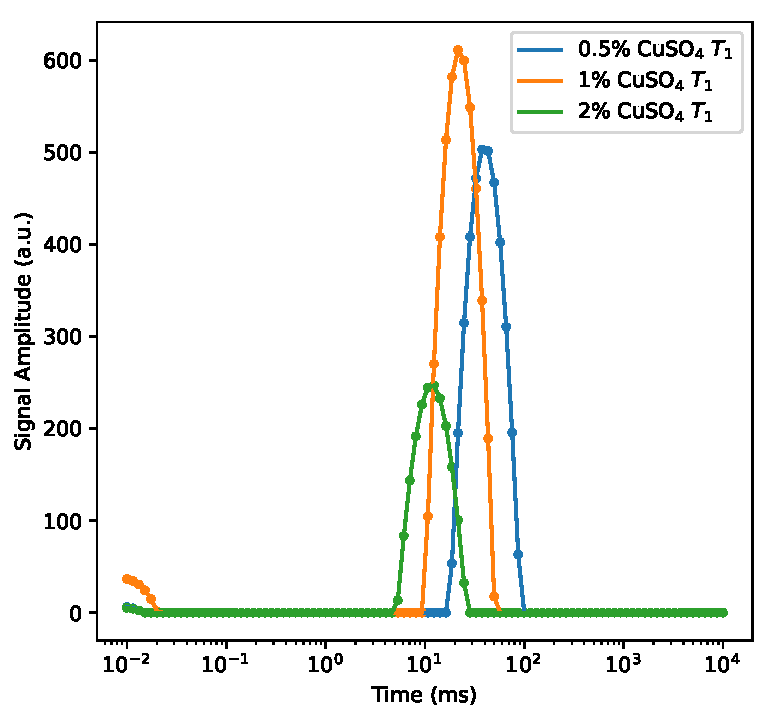
\includegraphics[width=\linewidth]{fig/T1all.pdf}   %以pic.jpg的0.5倍大小输出
    \end{minipage}
  }
  \subfigure[横向弛豫时间$T_2$] %第二张子图
  {
    \begin{minipage}[b]{0.48\linewidth}
      \centering      %子图居中
      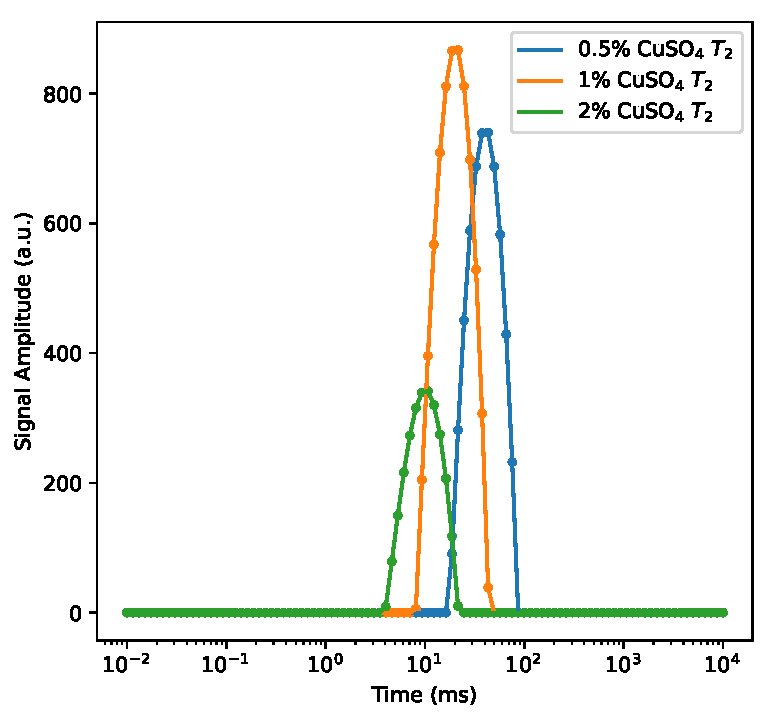
\includegraphics[width=\linewidth]{fig/T2all.pdf}   %以pic.jpg的0.5倍大小输出
    \end{minipage}
  }
  \caption{不同浓度的CuSO$_4$溶液对弛豫时间的影响}
  \label{fig:diff_delaytime}
\end{figure}
\subsection{核磁共振成像}
按照软件说明书的指示,用0.5\%CuSO$_4$溶液做样品,进行Prescan,再用Scout定位,软件能够自动校准中心频率,其余参数保持默认即可。随后分别用三角柱、四方柱、六角柱放入溶液成像。成像结果如\autoref{figure:NMRI} 所示。核磁共振实际上测量的是水分子中氢核的信号,由于样品中不含水,因此样品所在位置没有核磁共振的信号,因此我们可以在核磁共振的图像上看到样品的形状。

\begin{figure}[]
  \centering 
  \subfigure[0.5\%CuSO$_4$+三角形样品]
  {
    \begin{minipage}[b]{0.31\linewidth}
      \centering
      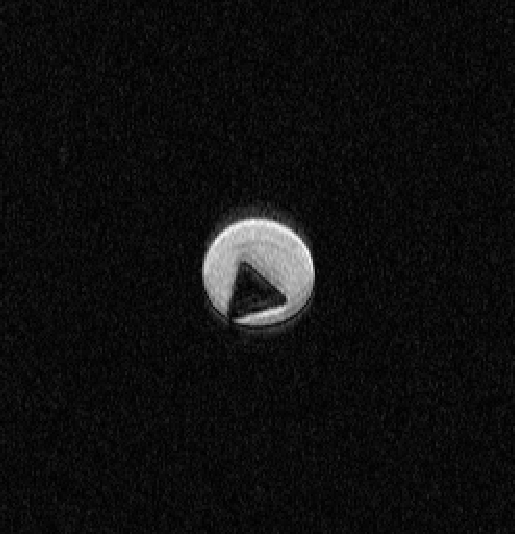
\includegraphics[width=\linewidth]{fig/0.5+triangle.PNG}
    \end{minipage}
  }
  \subfigure[0.5\%CuSO$_4$+正方形样品]
  {
    \begin{minipage}[b]{0.31\linewidth}
      \centering 
      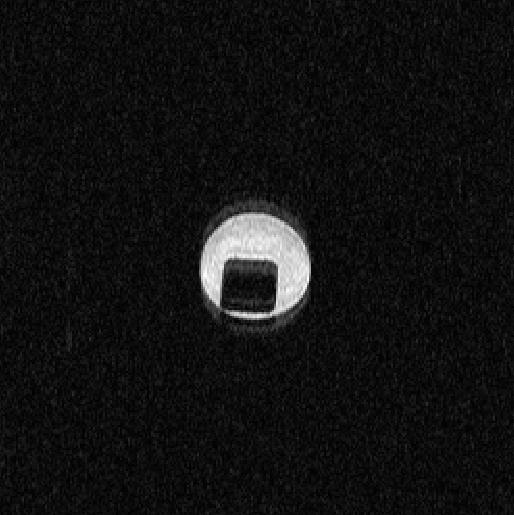
\includegraphics[width=\linewidth]{fig/0.5+square.PNG}
    \end{minipage}
  }
  \subfigure[0.5\%CuSO$_4$+六边形样品]
  {
    \begin{minipage}[b]{0.31\linewidth}
      \centering   
      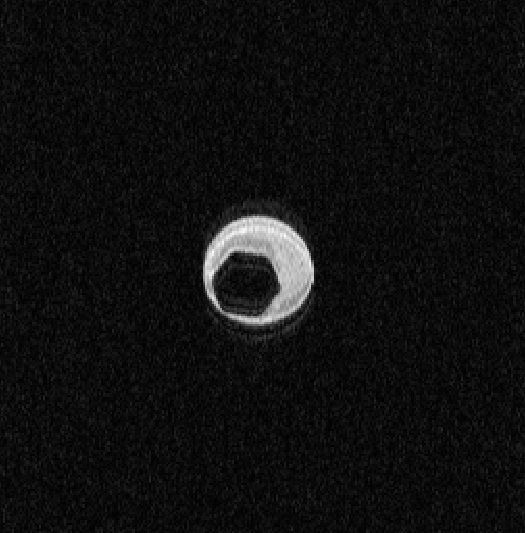
\includegraphics[width=\linewidth]{fig/0.5+hexagon.PNG} 
    \end{minipage}
  }
  \caption{0.5\%CuSO$_4$溶液放入不同形状样品后的核磁共振图像}
  \label{figure:NMRI} 
\end{figure}
\autoref{figure:NMRI} 不容易看出溶液浓度对于成像的影响,因此我们将装有0.5\%CuSO$_4$溶液的小试管放入装有1\%和2\%的CuSO$_4$溶液的大试管中,进行核磁共振成像,得到成像结果如\autoref{figure:NMRI2} 所示。
\begin{figure}[]
  \centering 
  \subfigure[0.5\%CuSO$_4$试管插入1\%CuSO$_4$试管]
  {
    \begin{minipage}[b]{0.31\linewidth}
      \centering
      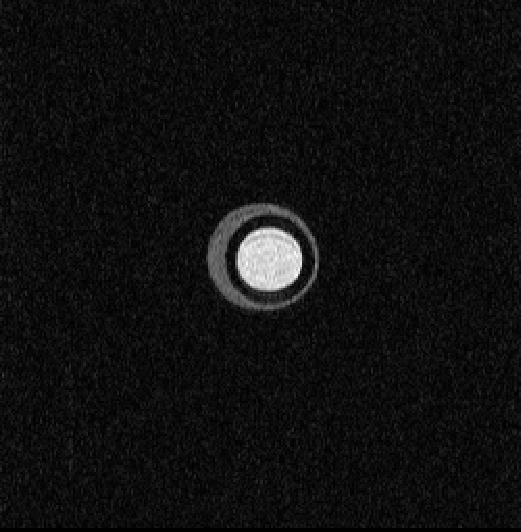
\includegraphics[width=\linewidth]{fig/0.5+1.PNG}
    \end{minipage}
  }
  \subfigure[0.5\%CuSO$_4$试管插入2\%CuSO$_4$试管]
  {
    \begin{minipage}[b]{0.31\linewidth}
      \centering 
      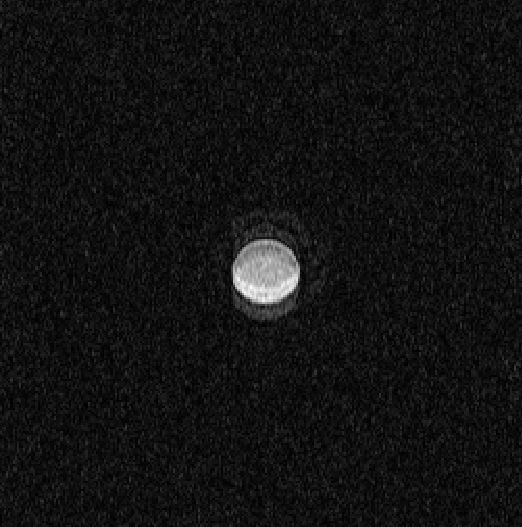
\includegraphics[width=\linewidth]{fig/0.5+2.PNG}
    \end{minipage}
  }
  \caption{浓度为0.5\%CuSO$_4$试管插入不同浓度试管的核磁共振图像}
  \label{figure:NMRI2} 
\end{figure}
可以看出,小试管中的部分信号强,而外面大试管中的信号弱。且CuSO$_4$的浓度越高,成像信号就越弱。下面我们对这个结果进行简要分析:硫酸铜溶液浓度越高,所提供的顺磁离子浓度越大,这会导致横向弛豫时间$T_2$减小。根据公式
	\begin{equation}
		S(t_x,t_y)\propto\iint e^{i(\omega_x t_x+\omega_y t_y)}\rho(x,y)e^{-\frac{t}{T_2}} {\rm d}x{\rm d}y
	\end{equation}
由上式可以看出,越小的弛豫时间会导致越小的被$T_2$加权的核密度$\rho(x,y,T_2)$,也就是说成像信号会越小,图像越暗。因此越高浓度的CuSO$_4$溶液对应的区域会越暗。这体现了$T_2$加权对于图像的影响,\autoref{figure:NMRI2} 体现了这一点,我们也可以通过这一特性判断样品顺磁离子的浓度。
\section{结论}
本实验使用苏州纽迈分析仪器股份有限公司生产的EDUMR20-015V-I型核磁共振成像技术实验仪,通过测定三种浓度的CuSO$_4$溶液(0.5\%,1\%,2\%)的弛豫时间$T_1$和$T_2$,深入探究了溶液浓度对弛豫时间的影响。同时,通过获取浸泡在CuSO$_4$溶液中不同形状样品的核磁共振图像,验证了$T_2$加权成像的原理。

这次实验使我们更深刻地理解了脉冲核磁共振和核磁共振成像的原理。通过实际操作,我们简单学习了核磁共振成像实验仪的基本操作,为将来在相关领域的研究和应用奠定了基础。通过对溶液浓度对弛豫时间的影响的研究,我们更好地了解了核磁共振技术在材料科学和生物医学领域的重要性。这次实验为我们提供了实践经验,有助于我们更深入地理解和应用核磁共振技术。
\begin{thebibliography}{}
  \bibitem{rabi1938new} Rabi, Isidor I., Zacharias, Jerrold R., Millman, Sidney, Kusch, Polykarp. (1938). A new method of measuring nuclear magnetic moment. \textit{Physical review. 53(4)}, 318.
  \bibitem{lauterbur1973image} Lauterbur, Paul C. (1973). Image formation by induced local interactions: examples employing nuclear magnetic resonance. \textit{Nature. 242(5394)}, 190-191.
  \bibitem{book} 吴思诚, 荀坤. (2015). 近代物理实验(第四版). 北京: 高等教育出版社.
\end{thebibliography}
  
\clearpage % 附录前另起一页
\appendix % 附录开始
\section{思考题}
\subsection{装着样品的圆形试管的一维剖面图应该是什么样子的曲线?}
装着样品的圆形试管的剖面图应该呈现出一条指数衰减曲线(自由感应衰减,FID曲线),但实际上会由于噪声等影响发生偏离。
\subsection{实空间图像的空间分辨率由什么因素决定?}
质子的浓度(即核磁矩的数密度)会直接影响核磁共振信号的强度。当质子浓度过低时,噪声可能会掩盖信号,导致图像分辨率降低。此外,样品中顺磁离子的浓度也会影响弛豫时间,进而影响图像分辨率。因为我们得到的图像是$T_2$加权的核密度,因此高浓度的顺磁离子会导致信号强度降低,也会使得图像分辨率降低。

除了上述因素,仪器的磁场均匀程度、编码时所选用的梯度场大小、仪器工作时的温度波动等因素也会对图像的空间分辨率产生影响。
\subsection{如何实现被$T_2$加权的核密度$\rho(x,y,T_2)$?}
如我们最后在实验中放入不同浓度的CuSO$_4$溶液成像一样,通过加入不同浓度的粒子,改变弛豫时间,即可实现被$T_2$加权的核密度$\rho(x,y,T_2)$。

\section{实验记录本}
实验记录本。
\end{document}
